\documentclass{beamer}
\usetheme{Montpellier}
\usepackage{verbatim}	
\usepackage{natbib}
\usepackage{comment}
\usepackage{amsmath}

\title{X-ray wave propagation }

\author{Sajid Ali\inst{1}}
% - Give the names in the same order as the appear in the paper.
% - Use the \inst{?} command only if the authors have different
%   affiliation.

\institute[NU] % (optional, but mostly needed)
{
  \inst{1}%
  Applied Physics\\
  Northwestern Univ}
% - Use the \inst command only if there are several affiliations.
% - Keep it simple, no one is interested in your street address.

\date{8 Aug 2018}
% - Either use conference name or its abbreviation.
% - Not really informative to the audience, more for people (including
%   yourself) who are reading the slides online

%\subject{Theoretical Computer Science}
% This is only inserted into the PDF information catalog. Can be left
% out. 

% If you have a file called "university-logo-filename.xxx", where xxx
% is a graphic format that can be processed by latex or pdflatex,
% resp., then you can add a logo as follows:

% \pgfdeclareimage[height=0.5cm]{university-logo}{university-logo-filename}
% \logo{\pgfuseimage{university-logo}}

% Delete this, if you do not want the table of contents to pop up at
% the beginning of each subsection:
\AtBeginSubsection[]
{
  \begin{frame}<beamer>{Outline}
    \tableofcontents[currentsection,currentsubsection]
  \end{frame}
}

% Let's get started
\begin{document}


\begin{frame}
  \titlepage
\end{frame}

\begin{frame}{Outline}
  \tableofcontents
  % You might wish to add the option [pausesections]
\end{frame}

% Section and subsections will appear in the presentation overview
% and table of contents.
\section{Wave propagation methods}

\subsection{Fresnel Propagation}

\begin{frame}{Fresnel Propagation}
  \begin{itemize}
  \item Approximation of the Huygens propagation.
  \item {Equation : $A(x) = \int_{-\infty}^{\infty}h_{space}(x,x^{'},k)t(x^{'})dx^{'}$}
  \footnote{$k = 2\pi/\lambda$ and $\lambda$ is the wavelength, primed co-ordinates denote source plane and unprime co-ordiantes denote observation plane }
  \footnote{\cite{Hanna2011}}
  \item {Kernel : $h_{space}(x,x^{'},k) = exp(i\frac{2\pi z}{\lambda})\sqrt{\frac{1}{i\lambda z}}exp(i\frac{\pi}{\lambda z}(x-x^{'})^2)$}

  
  \end{itemize}
\end{frame}

\subsection{Fraunhofer Propagation}

\begin{frame}{Fraunhofer Propagation}
\begin{itemize}
	\item Further approximation of the Huygens propagation valid at very large propagation distances.
	\item Valid when $\frac{W^{2}}{L\lambda}<<1$ or Fresnel number, $N_{F}<<1$
	\footnote{Fresnel Number is defined as $N_{F}=\frac{a^{2}}{\lambda L}$, where $a$ is the aperture, $L$ is the distance of propagation and $\lambda$ is the wavelength.}
  \item {Equation : $A(x) = \int_{-\infty}^{\infty}\psi(x^{'})\exp(i2\pi\frac{xx^{'}}{\lambda z})dx^{'}$}
	\item This can be seen as a scaled Fourier Transform and implemented using FFT.

\end{itemize}
\end{frame}

\begin{frame}{Fraunhofer propagator - accuracy\footnote{Green plots represent the result of the propagator and blue ones represent the results of exact evaluation }}
\begin{center}
	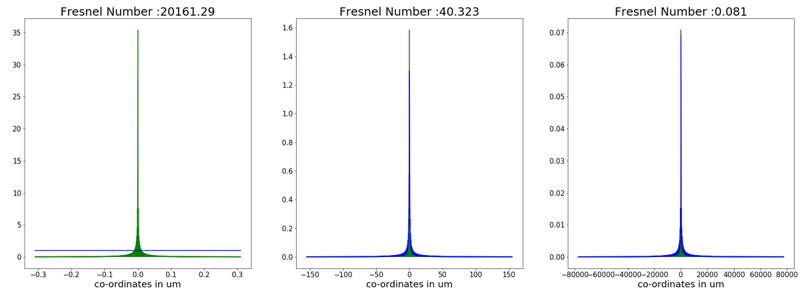
\includegraphics[scale=0.5]{ff}
\end{center}
\end{frame}


\subsection{Fresnel Integral: Evaluation Methods}
\begin{frame}{Evaluation Methods}
\begin{itemize}
	\item {Direct computation}
	\item {Spectral methods}
\end{itemize}
\end{frame}

\begin{frame}{Fresnel Propagation : Direct computation}
\begin{itemize}
	\item Naive method : $A(x) = \frac{\delta X}{\sqrt{j\lambda z}} exp( \frac{j\pi x^{2}}{\lambda z})\left\{\sum_{n=1}^{\infty}U_{n}exp(\frac{j\pi X_{n}^{2}}{\lambda z})exp(\frac{-j2\pi xX_{n}}{\lambda z})\right\}$ \footnote{\cite{Kelly2014}} 
	\item Complexity is $O(N^{2})$ (assuming length of input and output arrays are the same)
	\item Rapidly oscillating quadratic phase factor forces use of large arrays.
	\item Advanced integral schemes have been developed to deal with the phase issue.\footnote{\cite{Koc2010}}
\end{itemize}
\end{frame}


\begin{frame}{Spectral Methods}
\begin{itemize}
	\item Approximations to the Fresnel integral that make use of the Fast Fourier Transform
	\item {They include the Transfer Function, Impulse Response and Single Fourier Transform methods.}
	\item {Each method is valid only in a small range}
\end{itemize}
\end{frame}

\begin{frame}{Transfer Function}
\begin{itemize}
	\item This method involves taking the FT of the signal and multiplying it with the "transfer function" in frequency space and finally applying an inverse FT to the product to bring it to real space. 
	\item Equation : $\mathcal{F}^{-1}(\mathcal{F}(f(x))H(fx))$
	\item Transfer fuction is $H(fx) = e^{jkz}exp(-j\pi\lambda z fx^{2})$
	\item Valid for small distances since as distance increases, the transfer function become undersampled\footnote{\cite{Voelz2009}}.
\end{itemize}
\end{frame}

\begin{frame}{Transfer Function propagator - accuracy\footnote{Green plots represent the result of the propagator and blue ones represent the results of exact evaluation }}
\begin{center}
	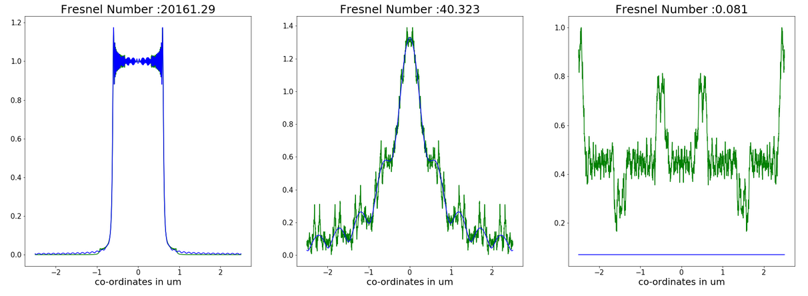
\includegraphics[scale=0.5]{tf}
\end{center}
\end{frame}

\begin{frame}{Impulse Response}
\begin{itemize}
	\item This method involves calcuating the "impulse response" in real space before taking transforming it to Fourier space and multiplying it with the input FT. This product is then brought back into real space by performing an inverse FT.
	\item Equation:
	$\mathcal{F}^{-1}(\mathcal{F}(f(x))\mathcal{F}(h(x)))$
	\item Impulse Response function is $h(x) = \frac{e^{jkz}}{jkz}exp(\frac{jk}{2\pi}x^{2})$
	\item Valid for large distances since as distance decrease, the impulse response function become undersampled\footnote{\cite{Voelz2009}}.
\end{itemize}
\end{frame}

\begin{frame}{IR - accuracy}
\begin{center}
	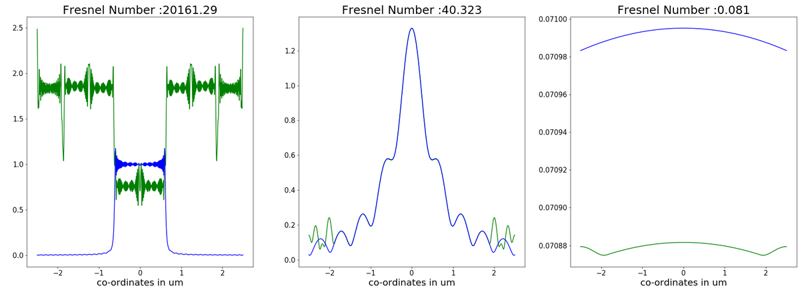
\includegraphics[scale=0.5]{ir}
\end{center}
\end{frame}


\begin{frame}{Fresnel Single Transform}
\begin{itemize}
	\item Modify the input wave by multiplying it with an input plane chirp function (quadratic phase factor) and take a fourier transform. Modify this with a second output plane chirp. 
		\item Equation:
	$\frac{e^{jkz}}{j\lambda z}exp(j\frac{k}{2z}x_2^{2})\mathcal{F}(f(x)exp(j\frac{k}{2z}(x_1^{2})))$
	\item {Valid for only one distance beacuse either the source plane chrip is undersampled or the output plane chirp is\footnote{\cite{Voelz2009}}. }
	\item Used when only amplitude is necessary and not the phase.
\end{itemize}
\end{frame}

\begin{frame}{Fresnel Single Transform propagator - accuracy\footnote{Green plots represent the result of the propagator and blue ones represent the results of exact evaluation }}
\begin{center}
	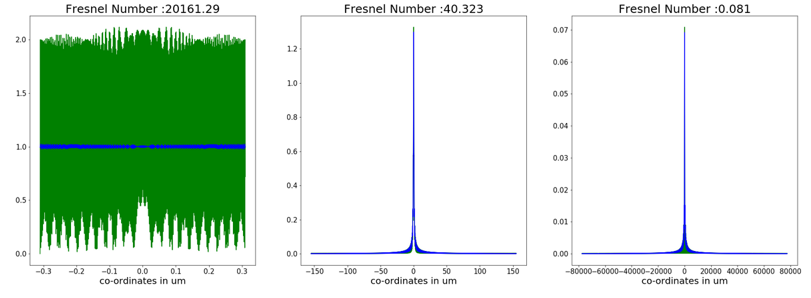
\includegraphics[scale=0.5]{fst}
\end{center}
\end{frame}


\subsection{Fractional Fourier Transform}
\begin{frame}{Fractonal Fourier Transform}
\begin{itemize}
	\item FrFT is a generalization of the Fourier Transform. The FT transforms a function from real space to frequency space. The FrFT can transform the function to anything in between. 
	
	\item $f_{a}(x) = \int_{-\infty}^{\infty}K_{a}(x,x^{'})f(x^{'})dx^{'}$\footnote{\cite{Hanna2011}}
	
	\item 
	$K_{a}(x,x^{'}) = \sqrt{\frac{1-icot(\alpha)}{2\pi}}exp(i0.5(x^{2}cot(\alpha)-2xx^{'}csc(\alpha)+x^{'}cot(\alpha)))$
	where $\alpha = \frac{\pi a}{2}$
	\item 	$K_{a}(x,x^{'}) = \delta(x\pm x^{'})$ when a is an odd/even multiple of $\pi$.

\end{itemize}
\end{frame}

\begin{frame}{Fresnel integral in terms of FrFT}
\begin{itemize}
	\item Fresnel integral can be stated in terms of Fractional Fourier Transform
	\item Given an input wave $t(x)$ Hanna et al,\footnote{\cite{Hanna2011}} examined the expression for Fresnel Transform and came up with the following mapping for the output wave:\\
	\begin{center}
		$A(x) = \sqrt{\frac{1}{1+itan(\alpha)}}*exp(i(\frac{2\pi L}{\lambda})^{2}tan(\alpha))$
		$exp[i0.25sin(2\alpha)(\frac{x}{L})^{2}]*t^{s}_{a}(\frac{x}{L}cos(\alpha))$
	\end{center}
	\item where $t^{s}$ is a scaled input wave given by $t(Lx)$ and $t_{a}^{s}(x)$ is the ath order Fractional Fourier transform ot $t^{s}(x)$ and $\alpha$, the order of the transform is given by $tan^{-1}(\frac{\lambda d}{2\pi L^{2}})$
	\item An alternate mapping first transforms the input and output wave to spherical references and describes the propagation between these spherical references via FrFT\footnote{\cite{Ozaktas95}}.
\end{itemize}
\end{frame}

\subsection{Linear Canonical Transform}
\begin{frame}{Linear Canonical Transform}
\begin{itemize}
	\item Fresnel Transform and FrFT are in fact just two specific cases of the more general Linear Canonical Transform. 
	\item The LCT is a an integral transform defined by three parameters $\alpha, \beta, \gamma$ as\footnote{\cite{Hennelly05}}
	\begin{center}
	$u_{\alpha, \beta, \gamma} = L_{\alpha, \beta, \gamma}{u(x)}(x^{'}) = exp(\frac{-j\pi}{4})\sqrt{\beta}\int_{-\infty}^{\infty}u(x)$
	$*exp[j\pi(\alpha x^{2} - 2\beta xx^{'} + \gamma x^{'2})]dx$
	\end{center}
	\item The LCT can be described by an abcd matrix which transform the Wigner Distribution as 
	$W(x,k) \rightarrow W(ax+bk,cx+dk)$ with relations between a,b,c,d that limiting them to three degrees of freedom. 
\end{itemize}
\end{frame}


\begin{frame}{LCT continued...}
\begin{itemize}
	\item The LCT acting in phase space is equivalent to a rotation in phase space according to\footnote{\cite{Hennelly05}}
	 \[
	\begin{bmatrix}
	x^{'}\\
	k^{'}
	\end{bmatrix} = 
	\begin{bmatrix}
	a & b \\
	c & d
	\end{bmatrix}
	\begin{bmatrix}
	x\\
	k
	\end{bmatrix}
	\]   
	\item The Fresnel transform is now described by the matrix\footnote{\cite{Hennelly05}}
	\[
	\begin{bmatrix}
		a & b \\
		c & d
	\end{bmatrix}
	=
	\begin{bmatrix}
	1 & \lambda z \\
	0 & 1
	\end{bmatrix}		
	\]
\end{itemize}
\end{frame}

\begin{frame}{Fresnel transform written as successive LCT's}
\begin{itemize}
	\item The Fresnel transform can be "decomposed" into a set of LCT's as two LCT's can be cascaded together. Two such methods are listed below.\footnote{\cite{Hennelly05}}
	\item Spectral Method (FFT, Chirp multiplication, FFT):
			\[
	\begin{bmatrix}
	1 & \lambda z \\
	0 & 1
	\end{bmatrix}
	=
	\begin{bmatrix}
	0 & -1 \\
	1 & 0
	\end{bmatrix}		
	\begin{bmatrix}
	1 & 0 \\
	-\lambda z & 1
	\end{bmatrix}	
	\begin{bmatrix}
	0 & 1 \\
	-1 & 0
	\end{bmatrix}			
	\]
	\item Direct Method (Chirp multiplication, optical Fourier Transform, Chirp multiplication ):
	\[
	\begin{bmatrix}
	1 & \lambda z \\
	0 & 1
	\end{bmatrix}
	=
	\begin{bmatrix}
	1 & 0 \\
	\frac{1}{\lambda z} & 1
	\end{bmatrix}	
	\begin{bmatrix}
	\lambda z & 0 \\
	0 & \frac{1}{\lambda z	}
	\end{bmatrix}			
	\begin{bmatrix}
	0 & 1\\
	-1 & 0
	\end{bmatrix}
		\begin{bmatrix}
	1 & 0 \\
	\frac{1}{\lambda z} & 1
	\end{bmatrix}	
	\]
	
\end{itemize}
\end{frame}

\begin{frame}{Fresnel Transform in terms of LCT}
\begin{itemize}
	\item Fresenl Transform is just a shear of the Wigner Distribution of the signal along the space co-ordinate.
\item The chirp convolution shears the signal's bandwidth which increases the sampling requirement. 
	\item When the sampling requiremnts for each operator are taken into account, any decomposition gives accurate results. The preferable methods are those that reduce the amount of up and downsampling of the signal.
\end{itemize}
\end{frame}

\subsection{Efficiency Xeon Phi}
\begin{frame}{FrFT on XeonPhi}
\begin{itemize}
	\item The newest cluster at ALCF is $\theta$ which has Xeon Phi nodes. Each Xeon Phi 7230 chip has 64 cores and $\approx$250 threads. Each core is lightweight but has AVX-512 enabled VPU. 
	\item Given that there are multiple methods to evaluate - sampling of FRFT, linear combination, eigenvalue decomposition, how do we pick one that's appropriate for Xeon Phi ? 
	\item To preseve properties like index additivity or prefer speed ? Does any method have benefits for the inverse problem? 
\end{itemize}
\end{frame}



%\begin{comment}
% Placing a * after \section means it will not show in the
% outline or table of contents.

\section*{Acknowledgements}

\begin{frame}{Acknowledgements}
  \begin{itemize}
  \item
    \alert{Chris Jacobsen} XSD, APS.
  \item
  	\alert{Kenan Li} SLAC National Accelerator Laboratory.
  \end{itemize}
\end{frame}

%\end{comment}

% All of the following is optional and typically not needed. 
%\appendix
\renewcommand*{\bibfont}{\small}
\section{References}
\begin{frame}[t, allowframebreaks]
\frametitle{References}
\bibliographystyle{alpha}
\bibliography{xray-prop}
\end{frame}

\end{document}

